\documentclass[a4paper,12pt]{article}

\usepackage[dutch]{babel}
\usepackage{fancyhdr}
\usepackage{graphicx}
\usepackage[pdftex,bookmarks=true]{hyperref}
\usepackage[utf8]{inputenc}
\usepackage{fullpage}
\usepackage{parskip}
\usepackage{float}
\usepackage{subcaption}
\usepackage{tabto}

\title{Samenvatting Onderzoekstechnieken \\ \large TIN 2 - HoGent}
\author{Lorenz Verschingel}

\begin{document}
\maketitle
\section{Het onderzoeksproces}
\subsection{De wetenschappelijke methode}
Aan de hand van \textbf{empirisch onderzoek} zijn we geïnteresseerd in volgende zaken:

\begin{enumerate}
\item Exploratie
\item Beschrijving
\item Voorspelling
\item Controle
\end{enumerate}

Het onderzoeksproces verloop normaal gezien als volgt:

\begin{enumerate}
\item Formuleren

Wat is de onderzoeksvraag
\item Exacte informatie behoefte definiëren

Welke specifieke vragen moeten we stellen
\item Uitvoeren onderzoek

Enquêtes, simulaties\dots
\item Verwerken gegevens

Statistische software
\item Analyseren gegevens

Uitvoeren statistische methodes
\item Conclusie schijven

Schrijven onderzoeksverslag
\end{enumerate}

\subsection{Basisconcepten in onderzoek}
\subsubsection{Variabelen en waarden}
Een variabele is een eigenschap van een object waardoor we objecten van elkaar kunnen onderscheiden.

Een waarde is een specifieke eigenschap, een invullen voor een variabele.

\subsubsection{Meetniveaus}
De kwalitatieve schalen zijn:

\NumTabs{6}
\begin{enumerate}
\item 	Nominaal:
		\tab{Categorieën}
		\tab{geslacht, ras, land\dots}
\item	Ordinaal:
		\tab{Volgorde}
		\tab{militaire rang, opleidingsniveau\dots}
\end{enumerate}

De kwantitatieve schalen zijn:
\NumTabs{6}
\begin{enumerate}
\item 	Interval:
		\tab{Meting: }
		\tab{nulpunt is onbelangrijk}
		\tab{graden Celsius}
\item	Ratio:
		\tab{Meting:}
		\tab{t.o.v. absoluut nulpunt}
		\tab{meter, Joule, kilogram}
\end{enumerate}

\subsubsection{Verbanden tussen variabelen}
Er is een verband tussen variabelen als hun waarde systematisch veranderen.

Men is vooral op zoek naar oorzakelijke verbanden:
\begin{itemize}
\item Frustratie leidt tot aggressie
\item Alcohol leidt tot minder oplettendheid
\end{itemize}
De oorzaak is hierbij de onafhankelijke variabele.

Het gevolg is de afhankelijke variabele.

Hierbij moet men wel opletten. Een verband tussen variabelen duidt niet noodzakelijk op een oorzakelijk verband.

\section{Analyse van 1 variabele}
\subsection{Beschrijvende statistiek}
\subsubsection{Centrummaten}
Het \textbf{gemiddelde} is de som van alle waarden gedeeld door het aantal waarden.

Om de \textbf{mediaan} te vinden, sorteert men de waarden en kiest men dan het middelste nummer.
Bij een even aantal getallen neemt men het gemiddelde van de twee middelste.

De \textbf{modus} is het vaakst voorkomende getal in een reeks getallen.
Als men niet onmiddellijk de modus kan aflezen kan men gebruik maken van ranges. Deze ranges zijn dan modale klassen.

\subsubsection{Spreidingsmaten}
Het \textbf{bereik} van een reeks getallen is de absolute waarde van het verschil tussen het grootste en het kleinste getal in de reeks: $|x_{min} - x_{max}|$

De \textbf{kwartielen} van een gesorteerde reeks getallen zijn de waarden die de lijst in vier gelijke delen verdeelt.
Elk deel vormt dus een kwart van de dataset.
Men spreekt van een eerste, tweede en derde kwartiel genoteerd als respectievelijk $Q_1$, $Q_2$, $Q_3$. Hierbij is $Q_2$ de mediaan.

De \textbf{variantie} is het gemiddelde gekwadrateerde verschil tussen de elementen van de dataset en zijn gemiddelde:
$\sigma^2 = \frac{1}{n}\sum^n_i (\mu-x_i)^2$

De \textbf{standaardafwijking} is hde vierkantswortel van de variantie.

\subsection{Eenvoudige grafieken}
\subsubsection{Cirkeldiagram}
Voordelen:
\begin{itemize}
\item Met percentages rond 20\% kan men makkelijk verduidelijken t.o.v. de volledige dataset.
\end{itemize}
Nadelen:
\begin{itemize}
\item Vergelijking op basis van de hoek.
\item De figuur wordt onduidelijk als er veel categorieën zijn.
\end{itemize}
Men gebruik best zo weinig mogelijk een cirkeldiagram.

\subsubsection{Staafdiagram}
Voordelen:
\begin{itemize}
\item Categorieën zijn makkelijk te vergelijken.
\item Per categorie zijn meerdere staven mogelijk.
\end{itemize}

\subsubsection{Boxplot}
Voordelen:
\begin{itemize}
\item Snelle manier om data te inspecteren en verschillende datasets te vergelijken.
\end{itemize}

\subsection{Interpretatie van grafieken}
\begin{figure}[H]
\centering
\begin{subfigure}{.49\textwidth}
  \centering
  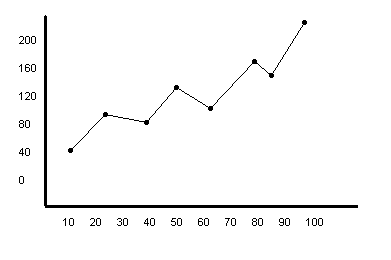
\includegraphics[width=.9\linewidth]{img/Hoofdstuk_2/data-ambiguiteit.png}
  \caption{Data-ambiguïteit}
  \label{fig:data-ambiguiteit}
\end{subfigure}
\begin{subfigure}{.49\textwidth}
  \centering
  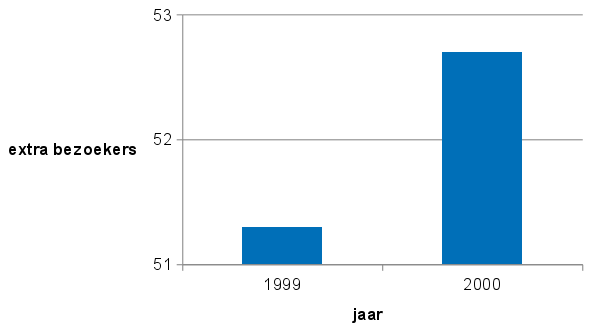
\includegraphics[width=.9\linewidth]{img/Hoofdstuk_2/data_distortion.png}
  \caption{Data distortion}
  \label{fig:datadistortion}
\end{subfigure}
\begin{subfigure}{.49\textwidth}
  \centering
  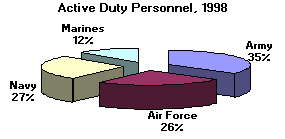
\includegraphics[width=.9\linewidth]{img/Hoofdstuk_2/data_distraction_1.png}
  \caption{Data distraction 1}
  \label{fig:datadistraction1}
\end{subfigure}
\begin{subfigure}{.49\textwidth}
  \centering
  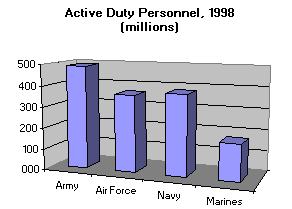
\includegraphics[width=.9\linewidth]{img/Hoofdstuk_2/data_distraction_2.png}
  \caption{Data distraction 2}
  \label{fig:datadistraction2}
\end{subfigure}
\caption{Valkuilen bij het interpreteren van grafieken}
\label{fig:ValkuilenGrafieken}
\end{figure}

\subsubsection{Data-ambiguïteit}
Data-ambiguïteit betekent vergeten aan te duiden wat de data betekent.
Zie figuur~\ref{fig:data-ambiguiteit}.

Enkele tips om dit te voorkomen:
\begin{itemize}
\item Benoem de assen
\item Geef een duidelijk titel
\item Benoem de meeteenheid (en evt. de grootorde)
\item Voeg een bijschrif toe met uitleg over de grafiek
\end{itemize}

\subsubsection{Data distortion}
Data distortion betekend dat men verkeerde conclusies kan trekken uit een grafische voorstelling.
Zie figuur~\ref{fig:datadistortion}: merk hierbij op dat de as niet op nul begint en er maar 3 waarden worden weergegeven.

\subsubsection{Data distraction}
Dit betekent dat de grafiek te veel toeters en bellen bevat.
Men moet de \textit{inkt to data ratio} beperken.
De figuren~\ref{fig:datadistraction1} en ~\ref{fig:datadistraction2} zijn hier voorbeelden van.

\end{document}